\subsection{Formal}
\label{sbsc:boundaries_formal}

Let's now turn to concrete definitions and bounds.
Remind that we are looking at the horizontal rectangle $\D$.

Suppose that $i_1 = i_2 \pmod 2$, $i_1$ is even.

\subsubsection{Bounds for $\D'$}

\begin{enumerate}[I.]
	\item Suppose both $\{\g_0(\M)\}$ and $\{\d_0(\M)\}$
	satisfy \ref{eq:cont-frac-left-normal} and the rectangle $\D$ is left-normal,
	that is, satisfies \ref{eq:left-normal}.
	We will denote such situation by $N-N-N$
	(segment $\D_1$ is left-normal, $\D_2$ is left-normal, rectangle $\D$ is normal).
	
	In this case define $\D'$ by equation
	\begin{equation}%\tag{11.9}
		\D' = f(\overline{21}3a_{i_1}... a_{i_2}3\overline{12}).
	\end{equation}
	
	\item[IIa.] Sets $\{\g_0(\M)\}$ and $\{\d_0(\M)\}$
	meet condition \ref{eq:cont-frac-left-normal}
	and $\D$ is left-shortened, that is, meets condition \ref{eq:left-shortened}.
	This is case $N-N-S$
	(segments $\D_1$ and $\D_2$ are left-normal, rectangle $\D$ is left-shortened).
	
	Then
	\begin{equation}\label{eq:bound-l-nns} %\tag{11.10}
		\D' = f(\overline{21}3a_{i_1}... a_{i_2}213\overline{12}).
	\end{equation}
	
	\item[IIb.] Set $\{\g_0(\M)\}$ meets \ref{eq:cont-frac-left-normal},
	$\{\d_0(\M)\}$ meets \ref{eq:cont-frac-left-shortened}.
	No matter, what takes place, \ref{left_shortened} of \ref{left_normal}.
	It is case $N-S$
	(segment $\D_1$ is left-normal, segment $\D_2$ left-shortened).
	Bound $\D_1$ is defined by \ref{eq:bound-l-nns}.
	
	\addtocounter{enumi}{1}
	\item Set $\{\g_0(\M)\}$ meets \ref{left_shortened_condition},
	$\{\d_0(\M)\}$ doesn't.
	In this ($Y-H$) case $\D'$ is defined by the following:
	\begin{equation}\tag{11.11}\label{bound_l_yh}
		\D' = f(\overline{21}312a_{i_1}... a_{i_2}3\overline{12}).
	\end{equation}
	
	\item Both $\{\g_0(\M)\}$ and $\{\d_0(\M)\}$
	meet \ref{left_shortened_condition}.
	In this ($Y-Y$) case $\D'$ is defined by
	\begin{equation}\tag{11.12}
		\D' = f(\overline{21}312a_{i_1}... a_{i_2}213\overline{12}).
	\end{equation}
\end{enumerate}

\begin{figure}[p]
	\centering
	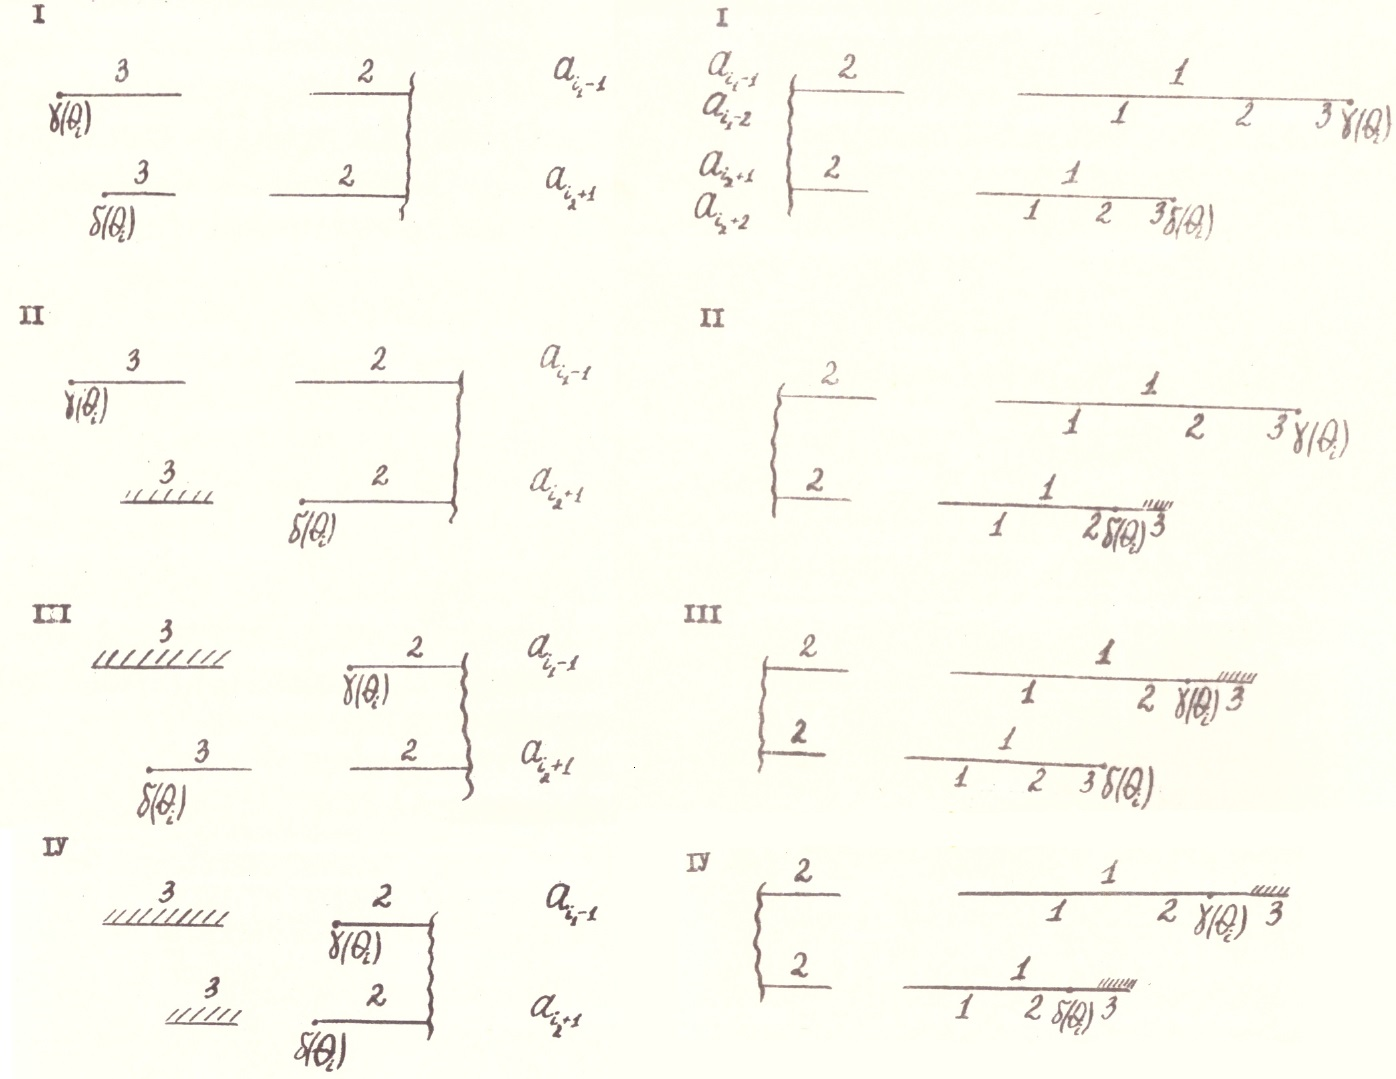
\includegraphics[width=0.9\textwidth]{pic1}
	\caption{Bounds $\D'$ (left) and $\D''$ (right).}
	\label{pic1}
\end{figure}

Figure \ref{pic1} illustrates the bounds. On the picture:

$\D_1' = \g(\T_i)$, $i=3,30$,
$\D_2' = \d  (\T_i)$, $i=3,30$,
$\D' = \D_1' + \D_2'$.

Hatched areas correspond to values of $a_{i_1 - 1}$ or $a_{i_2 + 1}$ (equal 3),
which can not appear in concrete case.

\subsubsection{Bounds for $\D''$}
Now we will provide formulas for $\D''$:

\begin{equation}\tag{11.13}
	\D'' = f(\overline{21}31a_{i_1}... a_{i_2}13\overline{12})
\end{equation}
\begin{equation}\tag{11.14}
	\D'' = f(\overline{21}31a_{i_1}... a_{i_2}1213\overline{12})
\end{equation}
\begin{equation}\tag{11.15}
	\D'' = f(\overline{21}3121a_{i_1}... a_{i_2}13\overline{12})
\end{equation}
\begin{equation}\tag{11.16}
	\D'' = f(\overline{21}3121a_{i_1}... a_{i_2}1213\overline{12})
\end{equation}

Figure \ref{table1} regulates the choise of the formulas.

\begin{figure}[ht]
	\centering
	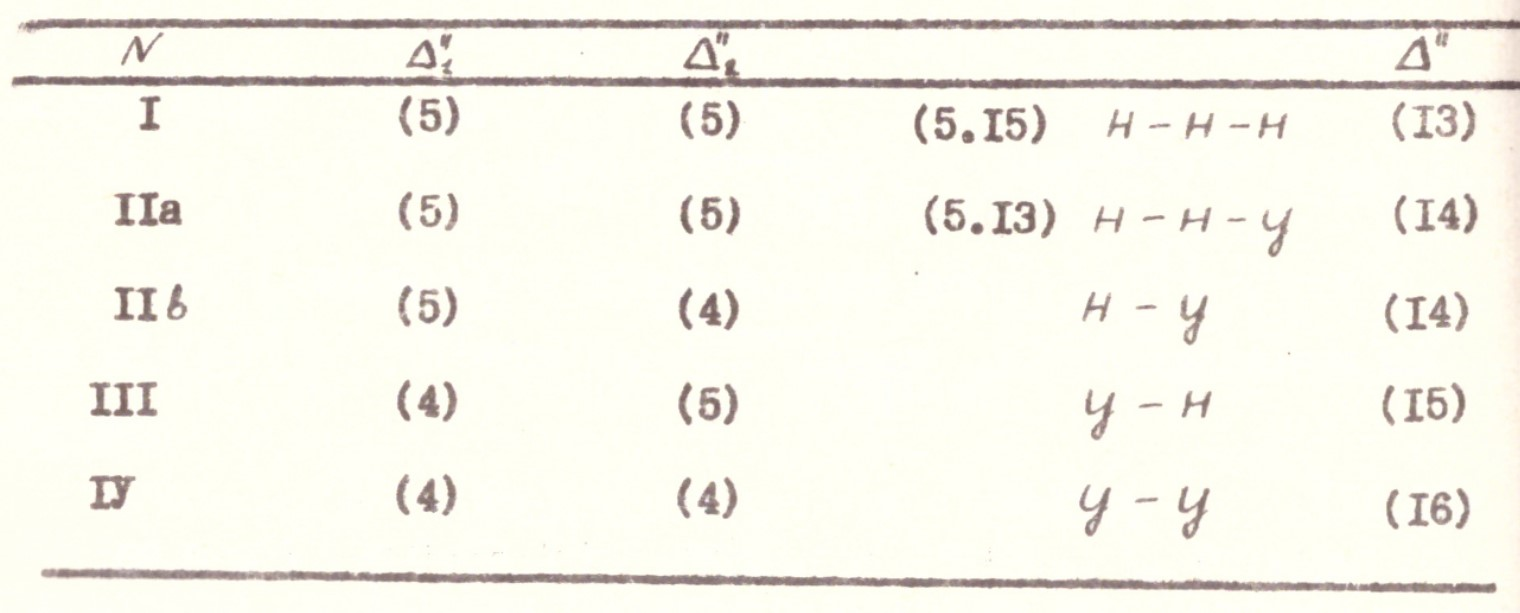
\includegraphics[width=0.8\textwidth]{table1}
	\caption{Rules for choose of $\D''$ in case $i_1 = i_2 \pmod 2$.}
	\label{table1}
\end{figure}

On the figure \ref{pic1}:
$\D_1'' = \g(\T_i)$, $i = 90, 94$,
$\D_2'' = \d  (\T_i)$, $i = 90, 94$,
$\D'' = \D_1'' + \D_2''$.
Hatched areas correspond to restricted value 3 of variables
$a_{i_1 - 2}$ or $a_{i_2 + 2}$.

\subsubsection{Case $i_1 \not\equiv i_2 \pmod 2$}

Now take case $i_1 \not\equiv i_2 \pmod 2$, $i_1$ is even. We will use rules from figure \ref{table2} to choose one of 4 formulas for $\D'$.

\begin{equation}\tag{11.17}
	I \hspace{15pt}
	\D' = f(\overline{21}3a_{i_1}... a_{i_2}13\overline{12})
\end{equation}
\begin{equation}\tag{11.18}
	II \hspace{15pt}
	\D' = f(\overline{21}3a_{i_1}... a_{i_2}1213\overline{12})
\end{equation}
\begin{equation}\tag{11.19}
	III \hspace{15pt}
	\D' = f(\overline{21}312a_{i_1}... a_{i_2}13\overline{12})
\end{equation}
\begin{equation}\tag{11.20}
	IV \hspace{15pt}
	\D' = f(\overline{21}312a_{i_1}... a_{i_2}1213\overline{12})
\end{equation}

\begin{figure}[ht]
	\centering
	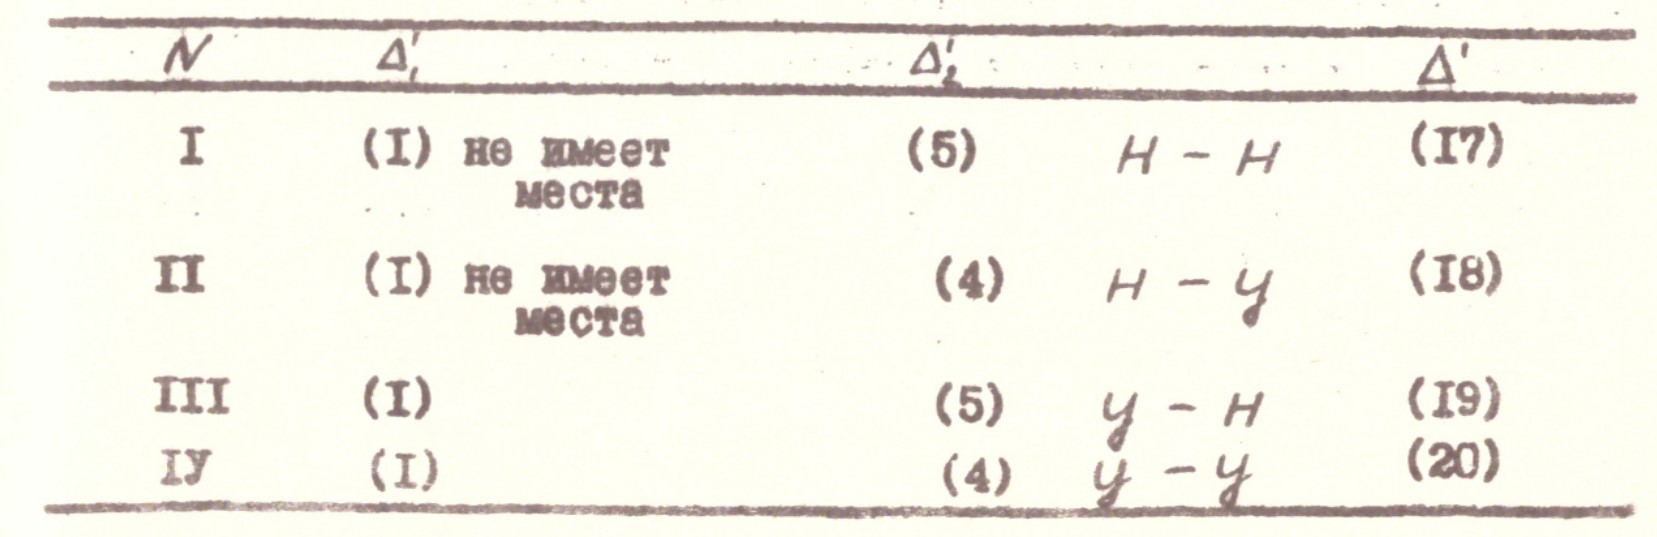
\includegraphics[width=0.8\textwidth]{table2}
	\caption{Rules for choose of $\D'$ in case $i_1 \ne i_2 \pmod 2$, $i_1$ is even.}
	\label{table2}
\end{figure}

To determine $\D''$ we will use rectangle
$$\{1, 0\}.$$
For this rectangle have $i_1 - 1 \equiv i_2 \pmod 2$, so we can use all the previous formulas to determine $\D''$.
